\documentclass{article}

\usepackage[colorlinks]{hyperref}
\usepackage{booktabs}
\usepackage{graphicx}
\usepackage[svgnames]{xcolor}
\usepackage{fancyvrb}

\usepackage[many]{tcolorbox}

% https://tex.stackexchange.com/questions/181082/how-to-reproduce-this-box-in-tcolorbox
\newtcbox{\srcbox}{
  enhanced,
  nobeforeafter,
  tcbox raise base,
  boxrule=0.4pt,
  top=0mm,
  bottom=0mm,
  right=0mm,
  left=4mm,
  arc=1pt,
  boxsep=2pt,
  before upper={\vphantom{dlg}},
  colframe=teal!75!white,
  coltext=teal!25!black,
  colback=teal!5!white,
  overlay={
    \begin{tcbclipinterior}
      \fill[teal!75!white] (frame.south west) rectangle node[text=white,font=\sffamily\bfseries\tiny,rotate=90] {SRC} ([xshift=4mm]frame.north west);
    \end{tcbclipinterior}
  }
}

\newtcolorbox{featurebox}[1]{colback=teal!5!white,colframe=teal!75!white,title={#1}}

\newtcolorbox{codebox}{colback=teal!5!white,colframe=teal!75!white}

% GitHub links
%\newcommand{\ghtag}{arch-doc}
\newcommand{\ghtag}{development}
\newcommand{\ghurlprefix}{https://github.com/quantum-bits/capernaum/blob/\ghtag}
\newcommand{\ghurl}[1]{\ghurlprefix/#1}
\newcommand{\ghsrc}[4]{
  \begin{tcolorbox}[
    skin=enhanced,
    after title={\hfill\textsf{source link}},
    colframe=blue!50!white,
    colback=blue!5!white,
    hyperurl=\ghurl{#3}/\#L#4,
    title={#1}]
    #2
  \end{tcolorbox}
}

% Names for things
\newcommand{\caper}{\textsc{Capernaum}}
\newcommand{\cli}{\textsc{Cli}}
\newcommand{\gh}{\textsc{GitHub}}
\newcommand{\rest}{\textsc{Rest}ful}
\newcommand{\unix}{\textsc{Unix}}
\newcommand{\linux}{\textsc{Linux}}

% Named URLs
\newcommand{\ansible}{\href{https://www.ansible.com/}{\textsc{Ansible}}}
\newcommand{\apollo}{\href{https://www.apollographql.com/}{\textsc{Apollo}}}
\newcommand{\axios}{\href{https://axios-http.com/}{\textsc{Axios}}}
\newcommand{\bg}{\href{https://www.biblegateway.com/}{Bible Gateway}}
\newcommand{\bull}{\href{https://www.npmjs.com/package/bull}{\textsc{Bull}}}
\newcommand{\cfse}{\href{https://www.taylor.edu/center-for-scripture-engagement/}{\textsc{C4se}}}
\newcommand{\cls}{\href{https://www.taylor.edu/center-for-scripture-engagement/survey/}{\textsc{Cls}}}
\newcommand{\dotenv}{\href{https://www.npmjs.com/package/dotenv}{\textsc{dotenv}}}
\newcommand{\gql}{\href{https://graphql.org/}{\textsc{GraphQL}}}
\newcommand{\grafana}{\href{https://grafana.com/grafana/}{\textsc{Grafana}}}
\newcommand{\handlebars}{\href{https://handlebarsjs.com/}{\textsc{Handlebars}}}
\newcommand{\jwt}{\href{https://jwt.io/}{\textsc{Jwt}}}
\newcommand{\nest}{\href{https://nestjs.com/}{\textsc{Nest}}}
\newcommand{\nginx}{\href{https://www.nginx.com/}{\textsc{nginx}}}
\newcommand{\nodemailer}{\href{https://nodemailer.com/}{\textsc{Node\-mailer}}}
\newcommand{\node}{\href{https://nodejs.org/}{\textsc{Node}}}
\newcommand{\pg}{\href{https://www.postgresql.org/}{\textsc{PostgreSQL}}}
\newcommand{\pmtwo}{\href{https://pm2.keymetrics.io/}{\textsc{Pm2}}}
\newcommand{\prometheus}{\href{https://prometheus.io/}{\textsc{Prometheus}}}
\newcommand{\qual}{\href{https://www.qualtrics.com/}{\textsc{Qualtrics}}}
\newcommand{\redis}{\href{https://redis.io/}{\textsc{Redis}}}
\newcommand{\ts}{\href{https://www.typescriptlang.org/}{\textsc{TypeScript}}}
\newcommand{\tu}{\href{https://www.taylor.edu/}{TU}}
\newcommand{\typeorm}{\href{https://typeorm.io/}{\textsc{TypeOrm}}}
\newcommand{\vega}{\href{https://vega.github.io/vega-lite/}{\textsc{Vega-Lite}}}
\newcommand{\vuetify}{\href{https://vuetifyjs.com/}{\textsc{Vuetify}}}
\newcommand{\vue}{\href{https://vuejs.org/}{\textsc{Vue}}}

%%% Local Variables:
%%% mode: latex
%%% TeX-master: "capernaum-architecture"
%%% End:

% LocalWords:  Capernaum Cli ful Ansible Axios se Cls GraphQL Grafana Jwt
% LocalWords:  Qualtrics TypeORM Vuetify


\title{\caper{} Architecture}
\author{Dr.\ Tom Nurkkala}

\begin{document}
\maketitle
\tableofcontents

\section{Introduction}
\label{sec:introduction}

\caper{} is a web-based system
that gathers responses to designated surveys taken at {\qual}.
When notified of a completed survey by a \qual{} web hook,
\caper{}
downloads the survey response
to its \pg{} relational database
using the
\qual{} \href{https://api.qualtrics.com/}{\rest{} API}.
\caper{} then
analyzes the response and
prepares a personalized analysis for the respondent:
a \LaTeX-formatted PDF containing both a text commentary
and graphical visualizations of results.
Finally, \caper{}
emails the PDF to the survey respondent.
Figure~\ref{fig:features} highlights additional
key features of the \caper{} architecture.

\begin{figure}
  \centering
  \begin{featurebox}{Key Architectural Features}
    \begin{enumerate}
    \item Administrative and registration apps implemented using
      the \vue{} framework and
      the \vuetify{} UI toolkit.
    \item Server software uses
      the \node-based
      server-side framework \nest.
    \item Implemented entirely in \ts.
    \item \gql{} API
      federates access to both relational data and an external \rest{} API.
      Uses \apollo{} \gql.
    \item Push notification to administrative application using
      \gql{}
      \href{https://www.apollographql.com/docs/react/data/subscriptions/}{subscriptions}.
    \item Distributed job queuing system
      using \bull{}
      and \redis.
    \item Command line interface (\cli) for administration, fixture loading, and testing.
    \item Production performance monitoring using \prometheus.
      Reporting and visualization via \grafana.
    \item Data persistence uses the
      \typeorm{} object-relational mapper,
      backed by a 
      \pg{} relational database.
    \item Report generation using \href{https://www.latex-project.org/}{\LaTeX} for typesetting
      and \vega{} to render charts.
      Reports delivered to survey respondents using \nodemailer.
    \item Template-based email notifications using \handlebars.
    \item Front end \nginx{} reverse proxy server.
    \item Run-time processes managed by \pmtwo.
    \item Configuration details maintained in environment variables
      using \dotenv.
    \item Integrated with
      \qual{} survey platform
      using inbound web hooks and the \qual{}
      \href{https://api.qualtrics.com/}{\rest{} API},
      which is accessed using \axios.
    \item Fully open source on \href{https://github.com/quantum-bits/capernaum.git}{\gh}.
    \end{enumerate}
  \end{featurebox}
  \caption{Key features of the \caper{} architecture.}
  \label{fig:features}
\end{figure}

The main customer for \caper{}
is the
Center for Scripture Engagement
(\cfse)
at Taylor University (\tu).
As part of a faith-based institution,
the \cfse{} publishes the
Christian Life Survey
(\cls)
at \qual.
\caper{} provides automated analysis and reporting on survey results
for individual respondents and
can also aggregate responses for groups of users.
As of November, 2021,
\caper{} has processed just over 19,000 surveys.
Refer to Table~\ref{tab:caper-stats} for additional statistics about \caper.

\begin{table}[h]
  \centering
  \begin{tabular}{lr}
    \toprule
    Initial Commit     & May, 2019      \\
    Production Release & December, 2019 \\
    \midrule
    Source files       & 356            \\
    Source lines       & 25,856         \\
    \midrule
    Reports processed  & 19,143         \\
    \bottomrule
  \end{tabular}
  \caption{\caper{} statistics (November, 2021).}
  \label{tab:caper-stats}
\end{table}

Traffic to the \cls{} is driven primarily by a partnership between \cfse{} and
\bg.
\bg{} is one of the top-three most-visited Christian web sites on the Internet.
In October, 2021, it was the
\href{https://www.similarweb.com/website/biblegateway.com/}{632-nd most visited site in the world,
  with 80~million visits}.
Although only a fraction of \bg{} users take the \cls,
the potential user volume is a key factor in the design of \caper.
In particular, \caper{} employs a distributed job queuing system
for survey analysis and report production,
designed to scale to handle 2,000 survey responses per minute.
This requirement is based on the \cfse{}'s
expectation that usage will grow significantly as \bg{}
begins actively promoting the \cls{} as planned.

\section{Architecture}
\label{sec:architecture}

Figure~\ref{fig:block-diagram}
presents a block diagram
of the \caper{} architecture.
\begin{figure}
  \centering
  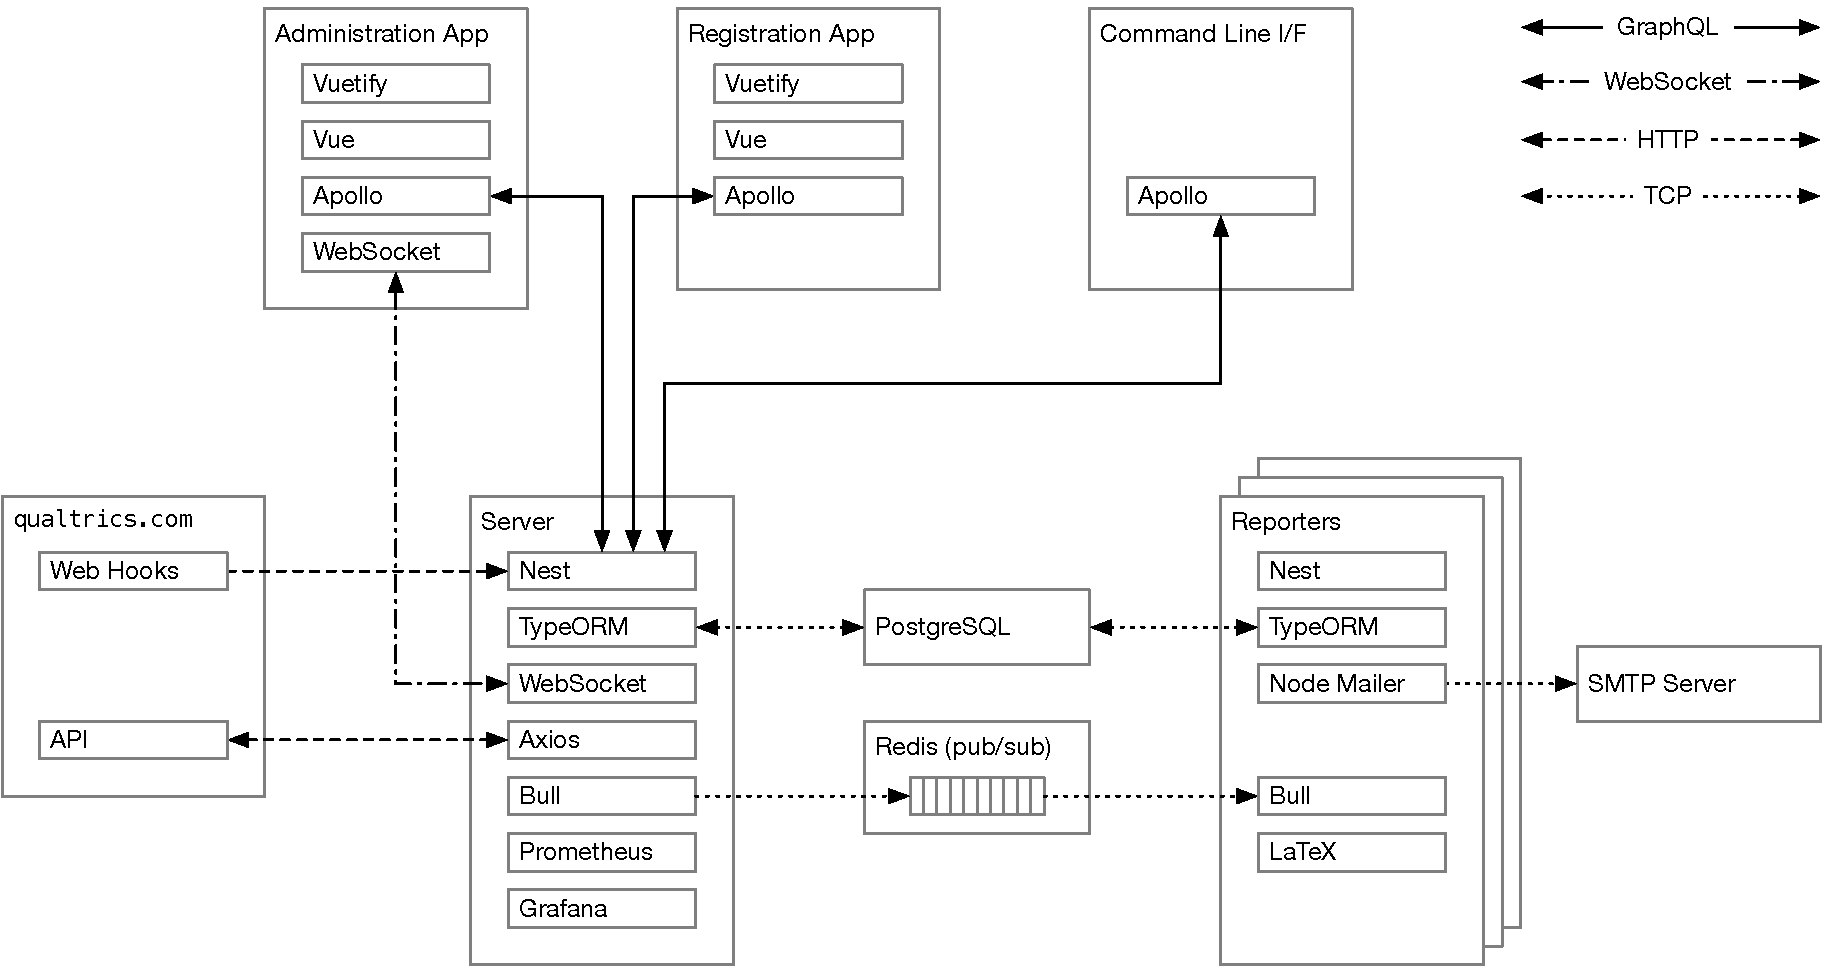
\includegraphics[width=\textwidth]{block-diagram}
  \caption{Block diagram of \caper.
    Communication between distributed processes is indicated in the legend.}
  \label{fig:block-diagram}
\end{figure}

\ghsrc{Source Code Link}{
  Throughout this document,
  these boxes
  link to a relevant location
  in the \caper{} source code.
  Click anywhere on the box to view the code
  on \textsc{GitHub}.
}{README.md}{1}

\subsection{Servers}
\label{sec:servers}

\caper{} employs two server processes,
an \hyperref[sec:application-server]{application server},
which provides the majority of \caper{} administrative functionality,
and a \hyperref[sec:reporting-server]{reporting server},
which generates reports and emails them to survey respondents.

Both servers are built atop the \nest{} application framework for \node.
\nest{} integrates many best-of-breed services and packages
in a coherent and performant
\href{https://www.martinfowler.com/articles/injection.html}{dependency-injection}
framework.
\ghsrc{Dependency Injection}{
  Injecting a repository into a database service.
}{server/apps/server/src/survey/services/survey.service.ts}{19}

\subsubsection{Application Server}
\label{sec:application-server}

The application server is the main server-side component in \caper.

\caper{} leverages \nest{}
to support its
\gql{} API,
\typeorm{} object-relational mapping, and
\pg{} database access and schema migration.
Using \ts{}
\href{https://www.typescriptlang.org/docs/handbook/decorators.html}{decorators},
a single class
can be annotated to serve as both
an object-relational \emph{entity}
and a \gql{} \emph{type}.
This design eliminates redundant and misaligned class definitions.
\ghsrc{\gql{} and Object-Relational Mapping}{
  Example of a class with decorators
  creating both database entities
  and \gql{} \href{https://graphql.org/learn/schema/}{types}.
}{server/apps/server/src/survey/entities/survey.ts}{12}

The application and reporting servers
communicate via a \bull{} job queue
which uses \redis{} publish-subscribe
for inter-process communication.
The two-server design allows multiple reporting servers to be spun up
to handle increased demand as usage scales up.
\ghsrc{Queue a Bull Job}{The reporter process
  exposes a service
  injected by the application server
  to queue a reporting job
}{server/apps/reporter/src/queue/queue.service.ts}{14}

When a respondent completes a survey,
\qual{} triggers a web hook
to notify \caper{} that a new survey
is ready to be processed.
\caper{}
exposes a small number of \rest{} endpoints
accessed by \qual{} for this purpose.
\ghsrc{Process \qual{} Web Hook}{
  The \texttt{QualtricsController} class
  exposes endpoints to \qual.
  The \texttt{completedResponse} method
  handles the \qual{} hook triggered
  when a respondent completes a survey.
  This method uses the \texttt{reportService}
  (injected by the class constructor)
  to queue a new job for the reporting server via \bull.
}{server/apps/server/src/qualtrics/qualtrics.controller.ts}{14}

As the application server processes various events from \qual,
it stores those events in the database for later inspection.
The server also dynamically pushes events to the
\hyperref[sec:admin-app]{admin app}
using a \gql{} subscription.
Push notifications via the subscription mechanism
allow an administrative user
to monitor activity on the \caper{} server
in near-real-time.
\ghsrc{Push Notifications}{
  This method saves a server-side event in the database
  and pushes the event to the administration app
  via a \gql{} subscription.
  \apollo{} implements subscriptions using a \websocket.
}{server/apps/server/src/events/event.service.ts}{21}

\caper{} exposes
a relevant subset of the \qual{} \rest{} API
to the rest of \caper.
\ghsrc{Consume \qual{} \rest{} API}{
  This dependency-injectable class
  gives access to all the \qual{} \rest{} endpoints
  needed by \caper.
}{server/libs/qualtrics-api/src/qualtrics-api.service.ts}{91}

The application server
uses the \texttt{QualtricsApiService}
for a variety of tasks, including these.
\begin{enumerate}
\item Retrieve surveys.
\item Retrieve survey results.
\item Establish and update \qual{} web hook endpoints.
\end{enumerate}
\ghsrc{Import a Survey}{
  As an example of the use of the API service,
  this method
  import a \qual{} survey
  (including all questions and available responses)
  into \caper{} for use in report generation.
}{server/apps/server/src/qualtrics/qualtrics.service.ts}{34}

Survey respondents can sign up to be part of a group,
which allows \caper{}
not only to report on individual survey responses
but also to aggregate group members' responses.
After a time limit for individual responses expires,
\caper{}
constructs a group report
and emails it to the administrator of the group.

\ghsrc{Maintain a Group}{
  The \texttt{GroupService}
  provides a \gql{} API
  that supports various group operations,
  including group maintenance
  and reporting.
}{server/apps/server/src/group/group.service.ts}{43}

Although the majority of \caper{}'s API surface
is based on \gql{},
it also exposes a few traditional \rest{} endpoints
to simplify integration third-party modules
that don't support \gql.
For example, the \caper{}
\hyperref[sec:admin-app]{administration app}
uses
\href{https://www.npmjs.com/package/filepond}{filepond}
to support uploaded images for reports.
\ghsrc{Upload and Retrieve Files}{
  The injectable \texttt{ImageController}
  implements standard HTTP support for uploading and downloading images.
  The endpoints it exposes are used by
  the \hyperref[sec:admin-app]{administration app}
  when creating or updating report content.
}{server/apps/server/src/image/image.controller.ts}{L24}

\caper{} uses \jwt{} for access control.
Administrative users authenticate
with an email address and password (stored encrypted in the \caper{} database)
and are issued a JSON Web Token (\jwt)
that is used for authorization throughout a session.
\ghsrc{Authenticate a User}{
  The authentication service verifies a user at login time
  and issues a \jwt{} for session control.
  Note the use of injected services for the user and \jwt.
}{server/apps/server/src/auth/auth.service.ts}{14}

\subsubsection{Reporting Server}
\label{sec:reporting-server}

The reporting server
(or servers)
consumes requests posted by
the application server to the \bull{} job queue.

\ghsrc{Service the Bull Job Queue}{
  \nest{} provides the \texttt{Process} decorator
  to configure a method to respond to queued jobs.
}{server/apps/reporter/src/daemon/queue.daemon.ts}{14}

The reporting server
creates the report for an individual survey
and emails the report to the respondent.

\ghsrc{Create and send a report}{
  The reporting server
  exposes a service that's injected into the job queue handler
  to process a single survey response.
}{server/apps/reporter/src/report/report.service.ts}{43}

In addition to reports for \emph{individual} survey respondents, 
\caper{} supports summary reports
for \emph{groups} of respondents.
\caper{} generates an individual report
when \qual{} invokes the appropriate web hook
upon a single respondent completing a survey.
A group report, however,
is created at a specific time,
determined in advance when a group is registered with \caper.
To schedule group report generation,
\caper{} uses the \href{https://www.npmjs.com/package/cron}{\texttt{cron}} module,
which was inspired by the standard \unix{} \texttt{cron} mechanism.
\ghsrc{Schedule Group Reports}{
  This class configures the \texttt{cron} module to fire as configured,
  retrieve details for any group whose scheduled reporting time has passed,
  and triggers group report generation and delivery.
}{server/apps/reporter/src/daemon/cron.daemon.ts}{11}

Each time the \texttt{cron} timer expires, \caper{} generates group reports.

\ghsrc{Process a Group Report}{
  This method triggers group report generation.
}{server/apps/reporter/src/report/report.service.ts}{116}

Both individual and group reports are generated
using \LaTeX{} and \vega{} to construct an attractive PDF.

\caper uses \vega{} to create charts based on survey response data
and writes those files to disk.

\ghsrc{Create Graphs using \vega}{
  Consistent with the
  dependency injection architecture
  used throughout \caper,
  we define \texttt{VisualizationService} as an injectable service.
  Each method constructs a \vega{} configuration
  object and then invokes
  the \texttt{makeChart} helper function
  that renders the visualization to a PDF file.
}{server/apps/server/src/visualization/visualization.service.ts}{8}

\caper{} writes \LaTeX{} sources
based on letter elements stored in the database
(created by the administrative user using the
\hyperref[sec:admin-app]{administration app}).
The generated \LaTeX{} includes
directives to embed the charts previously created.

\ghsrc{Create \LaTeX{} Source}{
  The \texttt{WriterService}
  includes a \texttt{render} method
  for each type of report element supported by \caper.
  The \texttt{renderAllElements} method
  iterates over letter elements retrieved from the database
  and invokes an element-specific method to generate a \LaTeX{} snippet.
  \caper collects these snippets
  into a single \LaTeX{} source file.
}{server/apps/server/src/writer/writer.service.ts}{188}

Finally, the reporting server
runs \LaTeX{} itself to produce a high-quality PDF
that is then sent to the respondent by email.

\ghsrc{Compile \LaTeX{} Source into a PDF}{
  This method writes the render \LaTeX{} source into a file
  that's then processed by invoking \texttt{latex}.
}{server/apps/server/src/writer/writer.service.ts}{567}

After constructing the PDF version of the report,
\caper{} sends it by email
to the survey respondent.

\ghsrc{Email a PDF Report to Respondent}{
  Construct an email that includes:
  \begin{enumerate}
  \item A greeting message
    written by the administrative user.
    \caper{} sends both an HTML and plain text version
    of the greeting message
    using MIME encoding.
  \item
    The PDF report as an attachment.
  \end{enumerate}
}{server/apps/server/src/mail/mail.service.ts}{12}

\subsection{Web Applications}
\label{sec:web-apps}

\caper{} implements two \vue-based ``single-page'' web applications.
The \hyperref[sec:admin-app]{Administrative App}
supports the \caper{} administrator,
and the \hyperref[sec:group-app]{Registration App}
primarily supports groups of survey respondents.

\subsubsection{Administrative Application}
\label{sec:admin-app}

\caper{} includes a \vue{}- and \vuetify{}-based
single-page
administrative web app.
The principal user of the admin app
is a person tasked with using \caper{}
to analyze and report on \qual{} surveys.
It allows such a user to:
\begin{enumerate}
\item
  Download the details of a survey from \qual{},
  either for the first time or to update \caper{} after a change is made to the survey on \qual{}
  (Figure~\ref{fig:manage-qualtrics}).

  \ghsrc{\qual{} Survey Management Page}{
    \vue{} component that implements survey management.
  }{ui-admin/src/pages/QualtricsPage.vue}{1}

  \begin{figure}
    \centering
    \screensnap{qualtrics}
    \caption{
      Manage \qual{} surveys.
      Provides details on imported surveys
      and whether a survey has been updated since its last import.
    }
    \label{fig:manage-qualtrics}
  \end{figure}
\item
  Create or edit a report (``letter'') to be associated with a survey
  (Figure~\ref{fig:letter-details}).

  \ghsrc{Individual Letter Details}{
    Top-level \vue{} component for letter management.
    Individual tabs within the interface are implemented as separate components.
  }{ui-admin/src/pages/letters/LettersPage.vue}{1}
  
  \begin{figure}
    \centering
    \screensnap{letter-details}
    \caption{
      Details of a report (letter), including email cover letter.
      All text ``areas'' (e.g., the cover letter)
      employ a \caper{} component that implements
      the \tiptap{} headless editing framework.
    }
    \label{fig:letter-details}
  \end{figure}

  The app provides a convenient drag-and-drop interface
  that allows the user to add, remove, and rearrange the various type of
  letter elements to be included in the report sent to survey respondents
  (Figure~\ref{fig:compose-letter}).

  \ghsrc{Letter Composition Tab}{
    Component that implements letter composition,
    including adding, removing, editing, and moving elements (using drag-and-drop).
  }{ui-admin/src/pages/letters/LetterContentTab.vue}{1}

  \begin{figure}
    \centering
    \screensnap{compose-letter}
    \caption{
      Composing a letter, showing an active drag operation.
      All letter components can be resequenced similarly.
      The context menu in each letter element (northeast corner of each box)
      contains a menu allowing additional letter elements to be inserted
      above or below each component.
    }
    \label{fig:compose-letter}
  \end{figure}
\item
  Upload and curate images to be used in report letters.
  \ghsrc{File Upload using \filepond}{
    \vue{} component that implements \filepond{}
    to support uploading images for inclusion in report letters.
  }{ui-admin/src/pages/ImagesPage.vue}{1}
\item
  View searchable data about survey responses gathered from \qual.
\item
  Manually trigger the creation and delivery of a report for a survey respondent
  for purposes of debugging or verification.
\item
  Manage \qual{} web hooks that trigger report generation
  (Figure~\ref{fig:manage-web-hooks}).

  \ghsrc{Manage \qual{} Web Hooks}{
    This page uses multiple embedded components to represent and maintain
    \qual{} web hooks.
  }{ui-admin/src/pages/webhooks/WebHooksPage.vue}{1}
  
  \begin{figure}
    \centering
    \screensnap{web-hooks}
    \caption{
      Manage \qual{} web hooks.
      \caper{} allows multiple servers to be configured (\textsf{Machines} section),
      with different web hooks set up for each (\textsf{Subscriptions} section).
    }
    \label{fig:manage-web-hooks}
  \end{figure}
\end{enumerate}

\subsubsection{Registration Application}
\label{sec:group-app}

Also a \vue{}- and \vuetify{}-based
single-page web app,
the \caper{} registration application
is a one-stop landing page that:

\begin{enumerate}
\item
  Allows individual users to access a configured survey directly.
\item
  Lets users who are participating with a group to enter their
  group code (Figure~\ref{fig:survey-landing-page}).
  This design allows the registration application
  to verity that the user has a valid group code
  before directing the user to \qual.
  \begin{figure}
    \centering
    \screensnap{survey-landing-page}
    \caption{
      Survey landing page.
      Users participating in a group
      enter their group code
      in the \textsf{Group Code} box,
      which is verified by the registration app
      before redirecting the user to \qual.
    }
    \label{fig:survey-landing-page}
  \end{figure}
\item
  Supports registration of groups,
  using a friendly ``stepper'' based wizard
  (Figure~\ref{fig:group-registration}).
  \begin{figure}
    \centering
    \screensnap{group-registration}
    \caption{
      Group registration page.
      To keep the interface simple,
      it is presented as a sequence of discrete steps
      using a \vue{} stepper component.
    }
    \label{fig:group-registration}
  \end{figure}
\end{enumerate}

\section{Data Model}
\label{sec:data-model-overview}

Figure~\ref{fig:summary-data-model}
shows an overview of the \caper{} data model.
A detailed model appears in Appendix~\ref{sec:detailed-data-model}.
\begin{figure}
  \centering
  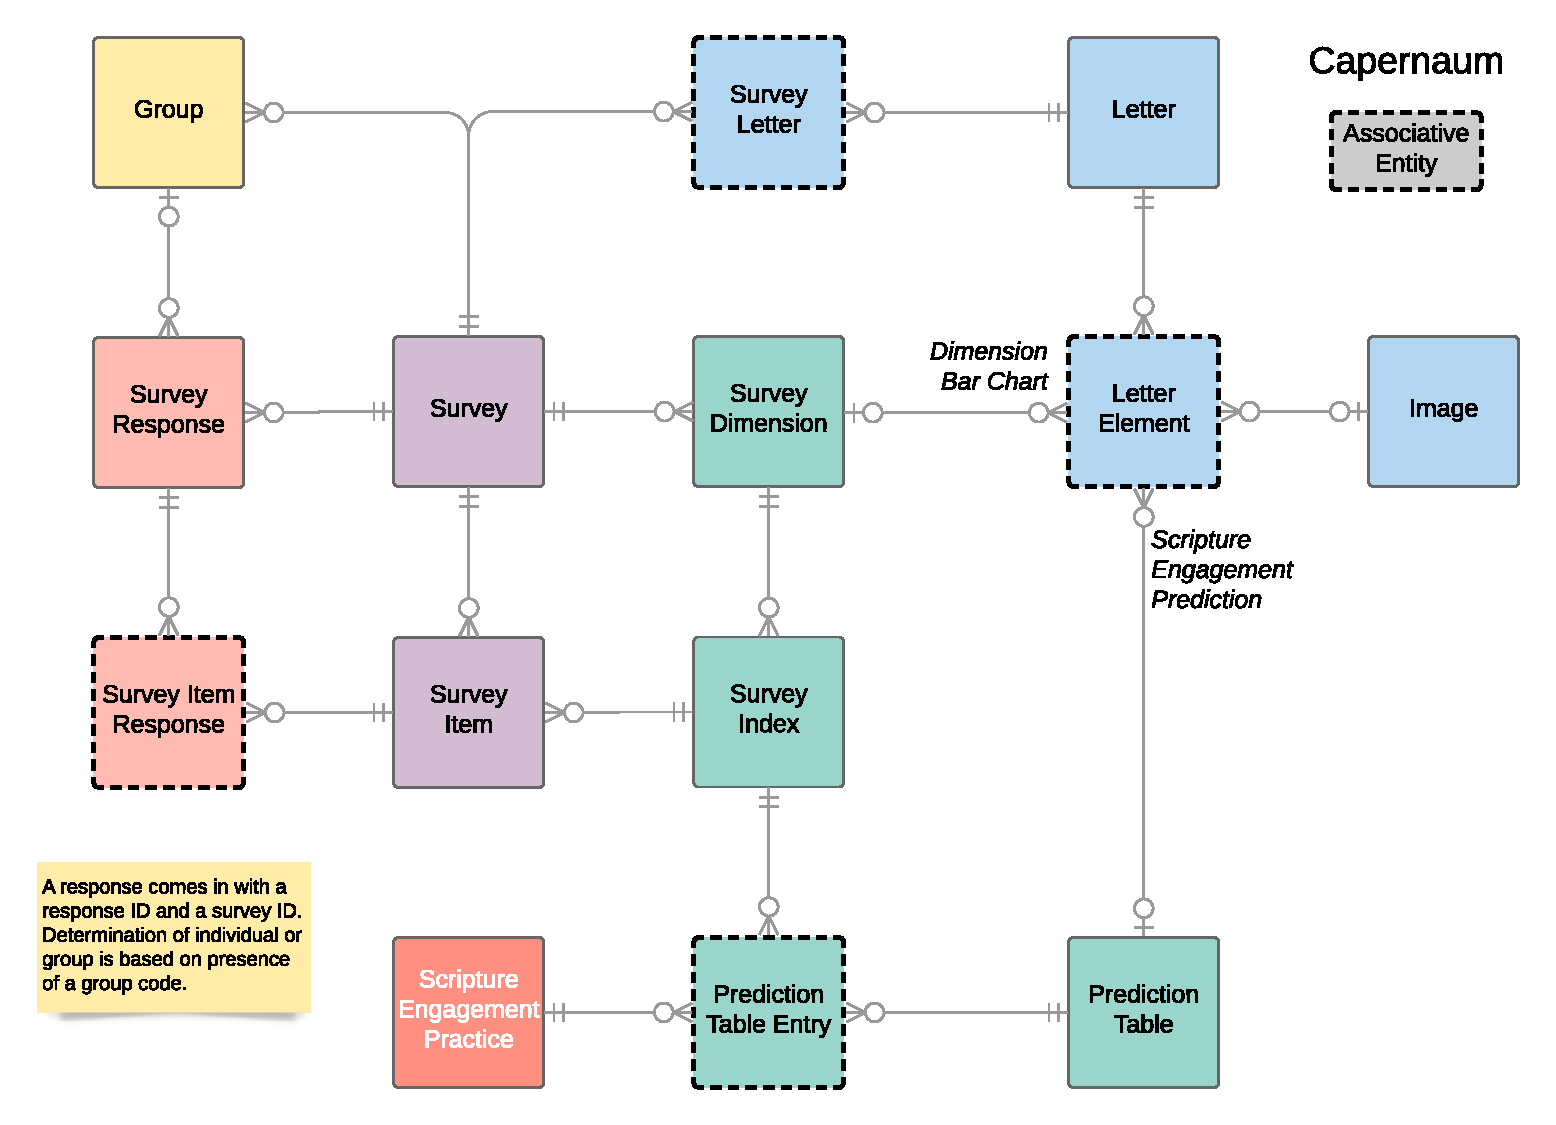
\includegraphics[width=\textwidth]{data-model-overview}
  \caption{Summary data model for \caper.}
  \label{fig:summary-data-model}
\end{figure}
Related tables are grouped by color
and serve the following purposes.
\begin{description}
\item[\textcolor{Violet}{Surveys (violet)}]
  The \texttt{Survey} and \texttt{SurveyItem} tables
  capture the details of a single survey on \qual.
\item[\textcolor{Salmon}{Survey Responses (salmon)}]
  The \texttt{SurveyResponse}
  and \texttt{Survey\-Item\-Re\-sponse}
  tables store the responses a single respondent
  makes to a survey.
\item[\textcolor{LightBlue}{Letters (light blue)}]
  Reports sent to survey respondents are called ``letters'' in the data model.
  Report content is entirely data driven and can be updated by a \caper's administrative user
  as desired for new surveys, new versions of a survey, or new report formats.
\item[\textcolor{Goldenrod}{Groups (gold)}]
  Survey respondents be members of a group of respondents
\item[\textcolor{LightGreen}{Users (green)}]
  Only administrative users need to log into \caper{} itself.
  It implements simple role-based security.
\end{description}

\section{Dev Ops}
\label{sec:dev-ops}

\caper{} is deployed on virtual servers
managed by Taylor University (\tu) Campus~IT.

\subsection{Configuration Management}
\label{sec:conf-management}

All run-time configuration is provided to \caper{} servers
as environment variables accessed
through the \node{} \texttt{process} object.
\caper{}
uses the \dotenv{} module,
which loads environment variables
from \texttt{.env} files at run time.
These \texttt{.env} files are constructed
as part of \hyperref[sec:deployment]{deployment and provisioning}.

\ghsrc{Define \emph{.env} File}{
  This \ansible{} template
  supplies the layout of the \texttt{.env} file
  used to configure the \hyperref[sec:application-server]{application server}.
}{ansible/templates/dot-env.server}{1}

\subsection{Deployment and Provisioning}
\label{sec:deployment}

\caper{} employs a fully-automated deployment
using \ansible,
which orchestrates a full \caper{} deployment to \linux,
including:
\begin{enumerate}
\item Add personal package archives (PPA's) to a vanilla Ubuntu load.
\item Install \linux{} packages using \texttt{apt}.
\item Create and configure a \texttt{capernaum} user with minimal permissions.
\item Provision \pg.
\item Clone the \caper{} source code from \gh.
\item Create \texttt{.env} files containing run-time configuration details.
\item Install \node{} modules required by all servers and apps.
\item Build all of \caper.
\item Provision the \pmtwo{} process manager.
\item Using \pmtwo, start the \caper{} \hyperref[sec:servers]{server processes}.
\item Provision \nginx.
\item Launch \nginx.
\end{enumerate}
\ghsrc{Provision using \ansible}{
  Complete YAML provisioning file.
}{ansible/provision.yaml}{1}

\subsection{Monitoring}
\label{sec:monitoring}

\caper{} uses \prometheus{}
for server-side monitoring.
In addition to the standard \linux{} metrics
gathered by default,
\caper{} implements an application-specific
counter for the number of emails sent.

\ghsrc{Define Custom \prometheus{} Counter}{
  Define a counter for to track the number of emails sent by \caper.
  Updated as part of report generation
  (individual and group).
}{server/apps/reporter/src/report/report.service.ts}{35}

\subsection{Process Management}
\label{sec:process-management}

With only a few server processes to manage,
\caper{} uses the \pmtwo{}
package for process control,
failover,
restart,
and logging.

\ghsrc{Configure \pmtwo}{
  Configure the application and reporting servers.
}{ansible/templates/ecosystem.config.js}{1}

\section{Command-Line Interface}
\label{sec:cli}

\caper{} includes a command-line interface (\cli)
that supports development, testing, and operations.
The \cli{} supports these operations:
\begin{enumerate}
\item Create an individual or group report.
\item Execute commands via the \qual{} \rest{} API.
\item Send individual or group reports by email.
\item Retrieve and list surveys from \qual.
\item Retrieve survey responses from \qual.
\item Invoke analytics processing on survey responses for testing.
\end{enumerate}

The \cli{} implements a \git-style, nested
command hierarchy.
Although powerful,
it can be easy to forget the details
of nested commands.
To remedy this problem,
the \cli's 
\texttt{hierarchy} command
displays a quick summary of all nested commands.
Figure~\ref{fig:cli-commands}
shows the command's output.

\ghsrc{Print Command Hierarchy}{
  Introspect all \cli{} commands recursively
  and generate a nicely-formatted, hierarchical list
  of all commands, flags, and options.
}{server/apps/cli/src/commands/hierarchy.ts}{1}

\begin{figure}
  \centering
\begin{Verbatim}[fontsize=\tiny,frame=single]
debug-cache
email
            test
env
fixture
            nuke --force --survey-id <survey-id>
gql
group
            close        group-pk
            force-report group-pk
            get          --with-responses code-word
            list         --open --ready
help
hierarchy   --verbose
letter
            group      letter-pk group-pk
            individual letter-pk survey_response-pk
            list
qualtrics
            org
            response
                         get --start-date --end-date survey-id response-id
            subscription
                         create --topic <name> publication-url survey-id
                         delete subscription-id
                         get    subscription-id
                         list
            survey
                         get  survey-id
                         list --by-date --all
report
            group      group-pk
            individual qualtrics-survey-id qualtrics-response-id
response
            dimension
                       group      ---pdf <pdf-file-name> --dimension <dimension-pk>
                       individual --pdf <pdf-file-name> --dimension <dimension-pk>
            import     survey-id
            msi
                       group
                       individual
            prediction
                       count      --pdf <pdf-file-name>
                       group
                       individual
            summarize
survey
            import  survey-id
            letters
            list
\end{Verbatim}
  \caption{Command summary generated by the \caper{} \cli}
  \label{fig:cli-commands}
\end{figure}

\appendix

\section{Detailed Data Model}
\label{sec:detailed-data-model}

Figure~\ref{fig:erd} shows the entity-relationship diagram for \caper's \pg{} database.
\begin{figure}
  \centering
  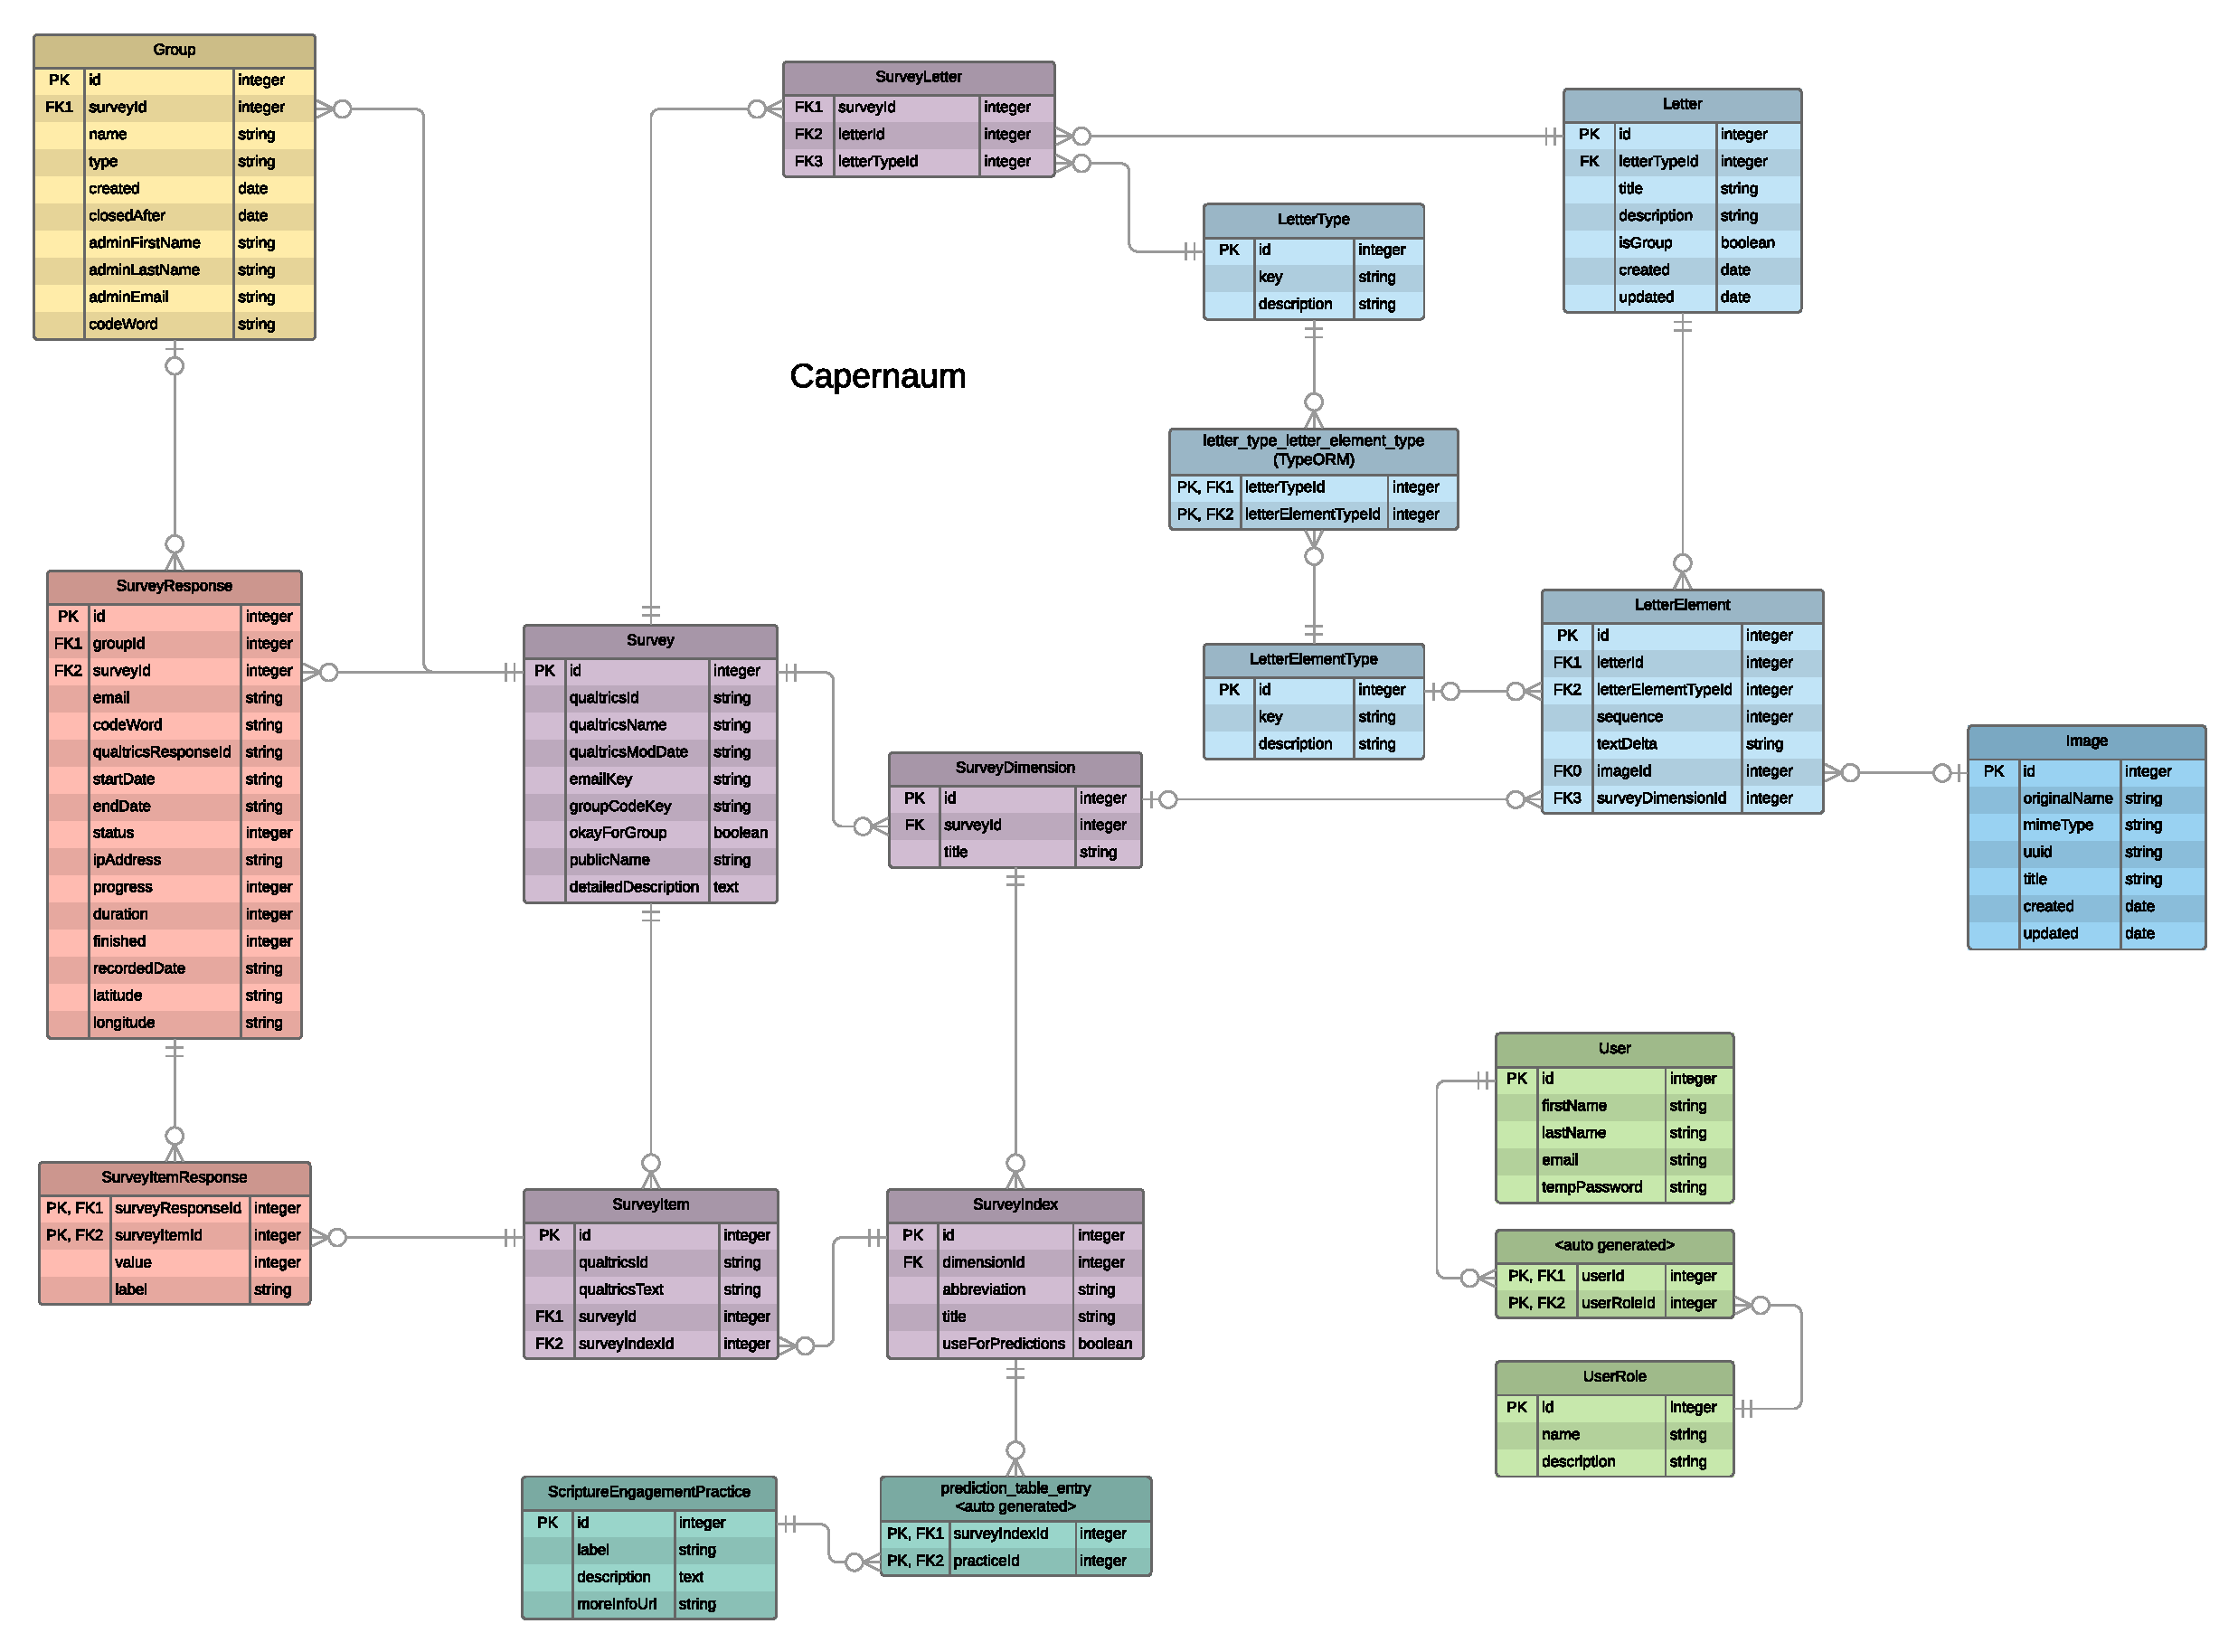
\includegraphics[width=\textwidth]{data-model}
  \caption{Entity-relationship diagram for \caper.}
  \label{fig:erd}
\end{figure}

\paragraph{\textcolor{Violet}{Surveys (violet)}}

The \texttt{Survey} and \texttt{SurveyItem} tables
capture the details of a single survey on \qual.
Using identifiers provided by \qual,
these tables allow \caper{} to perform the statistical analysis at the heart of each report letter.
To support statistical analysis,
\caper{} allows survey questions to be grouped into a category hierarchy.
Each survey question (\texttt{SurveyItem})
can be grouped into a \texttt{SurveyIndex},
which can in turn be grouped into a \texttt{SurveyDimension}.
\caper{} uses the latter entity to calculate aggregate attitudes
toward characteristics measured by the survey instrument itself.

\paragraph{\textcolor{Salmon}{Survey Responses (salmon)}}

The \texttt{Survey\-Res\-ponse}
and \texttt{Survey\-Item\-Res\-ponse}
tables store the responses a single respondent
makes to a survey.
\texttt{Survey\-Res\-ponse} is related to a survey
and has one associated \texttt{SurveyItemResponse}
for each \texttt{SurveyItem}.

\paragraph{\textcolor{LightBlue}{Letters (light blue)}}

Reports sent to survey respondents are called ``letters'' in the data model.
Report content is entirely data driven and can be updated by a \caper's administrative user
as desired for new surveys, new versions of a survey, or new report formats.

Each \texttt{Letter} contains multiple
instances of a \texttt{Letter\-Ele\-ment}.
A \texttt{Letter\-Ele\-ment} has an associated type
(e.g., boilerplate text,
uploaded image,
graph of analytical results).

\caper{} can report results for individual survey respondents
and can also aggregate results for people who identify as part of a group.
The \texttt{LetterType} entity enforce this distinction
and also partitions the types of letter elements,
allowing the user interface to present only valid \emph{element} types
for each \emph{letter} type.

\paragraph{\textcolor{Goldenrod}{Groups (gold)}}

Survey respondents can indicate membership in a group of respondents
(e.g., members of a church, students in a course).
Each \texttt{Group} entity stores the detail of one group
and will be associated with a \texttt{SurveyResponse}
when the respondent enters his or her group code
prior to taking the survey.

\paragraph{\textcolor{LightGreen}{Users (green)}}

Because only a few administrative users have a need to log into \caper{} itself,
its user management is quite modest.
There is a many-to-many relationship between \texttt{User} and \texttt{User Role},
allowing for conventional role-based access control.

A \texttt{User} authenticates with an email address and password.
Passwords are stored in encrypted form in the database.
One a user logs in,
access is granted using a
JSON Web Token (\jwt)
that enumerates each \texttt{UserRole} for which the \texttt{User} is authorized.

\texttt{UserRole} data are employed to control access to views
in the administrative application in the browser
as well as \gql{} and \rest{} API access on the server.


\end{document}

%%% Local Variables:
%%% mode: latex
%%% TeX-master: t
%%% End:

% LocalWords:  Ansible Qualtrics nd lr SurveyItem SurveyIndex UserRole README
% LocalWords:  SurveyDimension SurveyResponse SurveyItemResponse LightBlue md
% LocalWords:  LetterElement LetterType LightGreen QualtricsController Dev env
% LocalWords:  completedResponse reportService filepond ImageController cron
% LocalWords:  QualtricsApiService GroupService VisualizationService makeChart
% LocalWords:  WriterService renderAllElements PPA's capernaum qualtrics ui
% LocalWords:  ansible sponse ponse Ele ment
